\subsubsection{Norm 3}\label{sec:norm3}
As previously mentioned, the \gls{chemcam} instrument consists of three spectrometers, each producing 2048 channels.
For data normalization, we follow the approach taken by the ChemCam team and normalize across individual spectrometers' wavelength ranges, a process known as \textit{Norm 3}~\cite{cleggRecalibrationMarsScience2017, andersonImprovedAccuracyQuantitative2017}.
This method ensures that the wavelength intensities captured by each spectrometer are normalized independently, thus preserving the relative intensities within each spectrometer.

Figure~\ref{fig:spectral_plot} shows a spectral plot of the \gls{ccs} data for the \textit{ultramafic} sample, illustrating the three distinct spectral regions, each captured by one of the three spectrometers.
Specifically, one spectrometer captures the \gls{uv} region, another captures the \gls{vio} region, and the third captures the \gls{vnir} region.

\begin{figure}
	\centering
	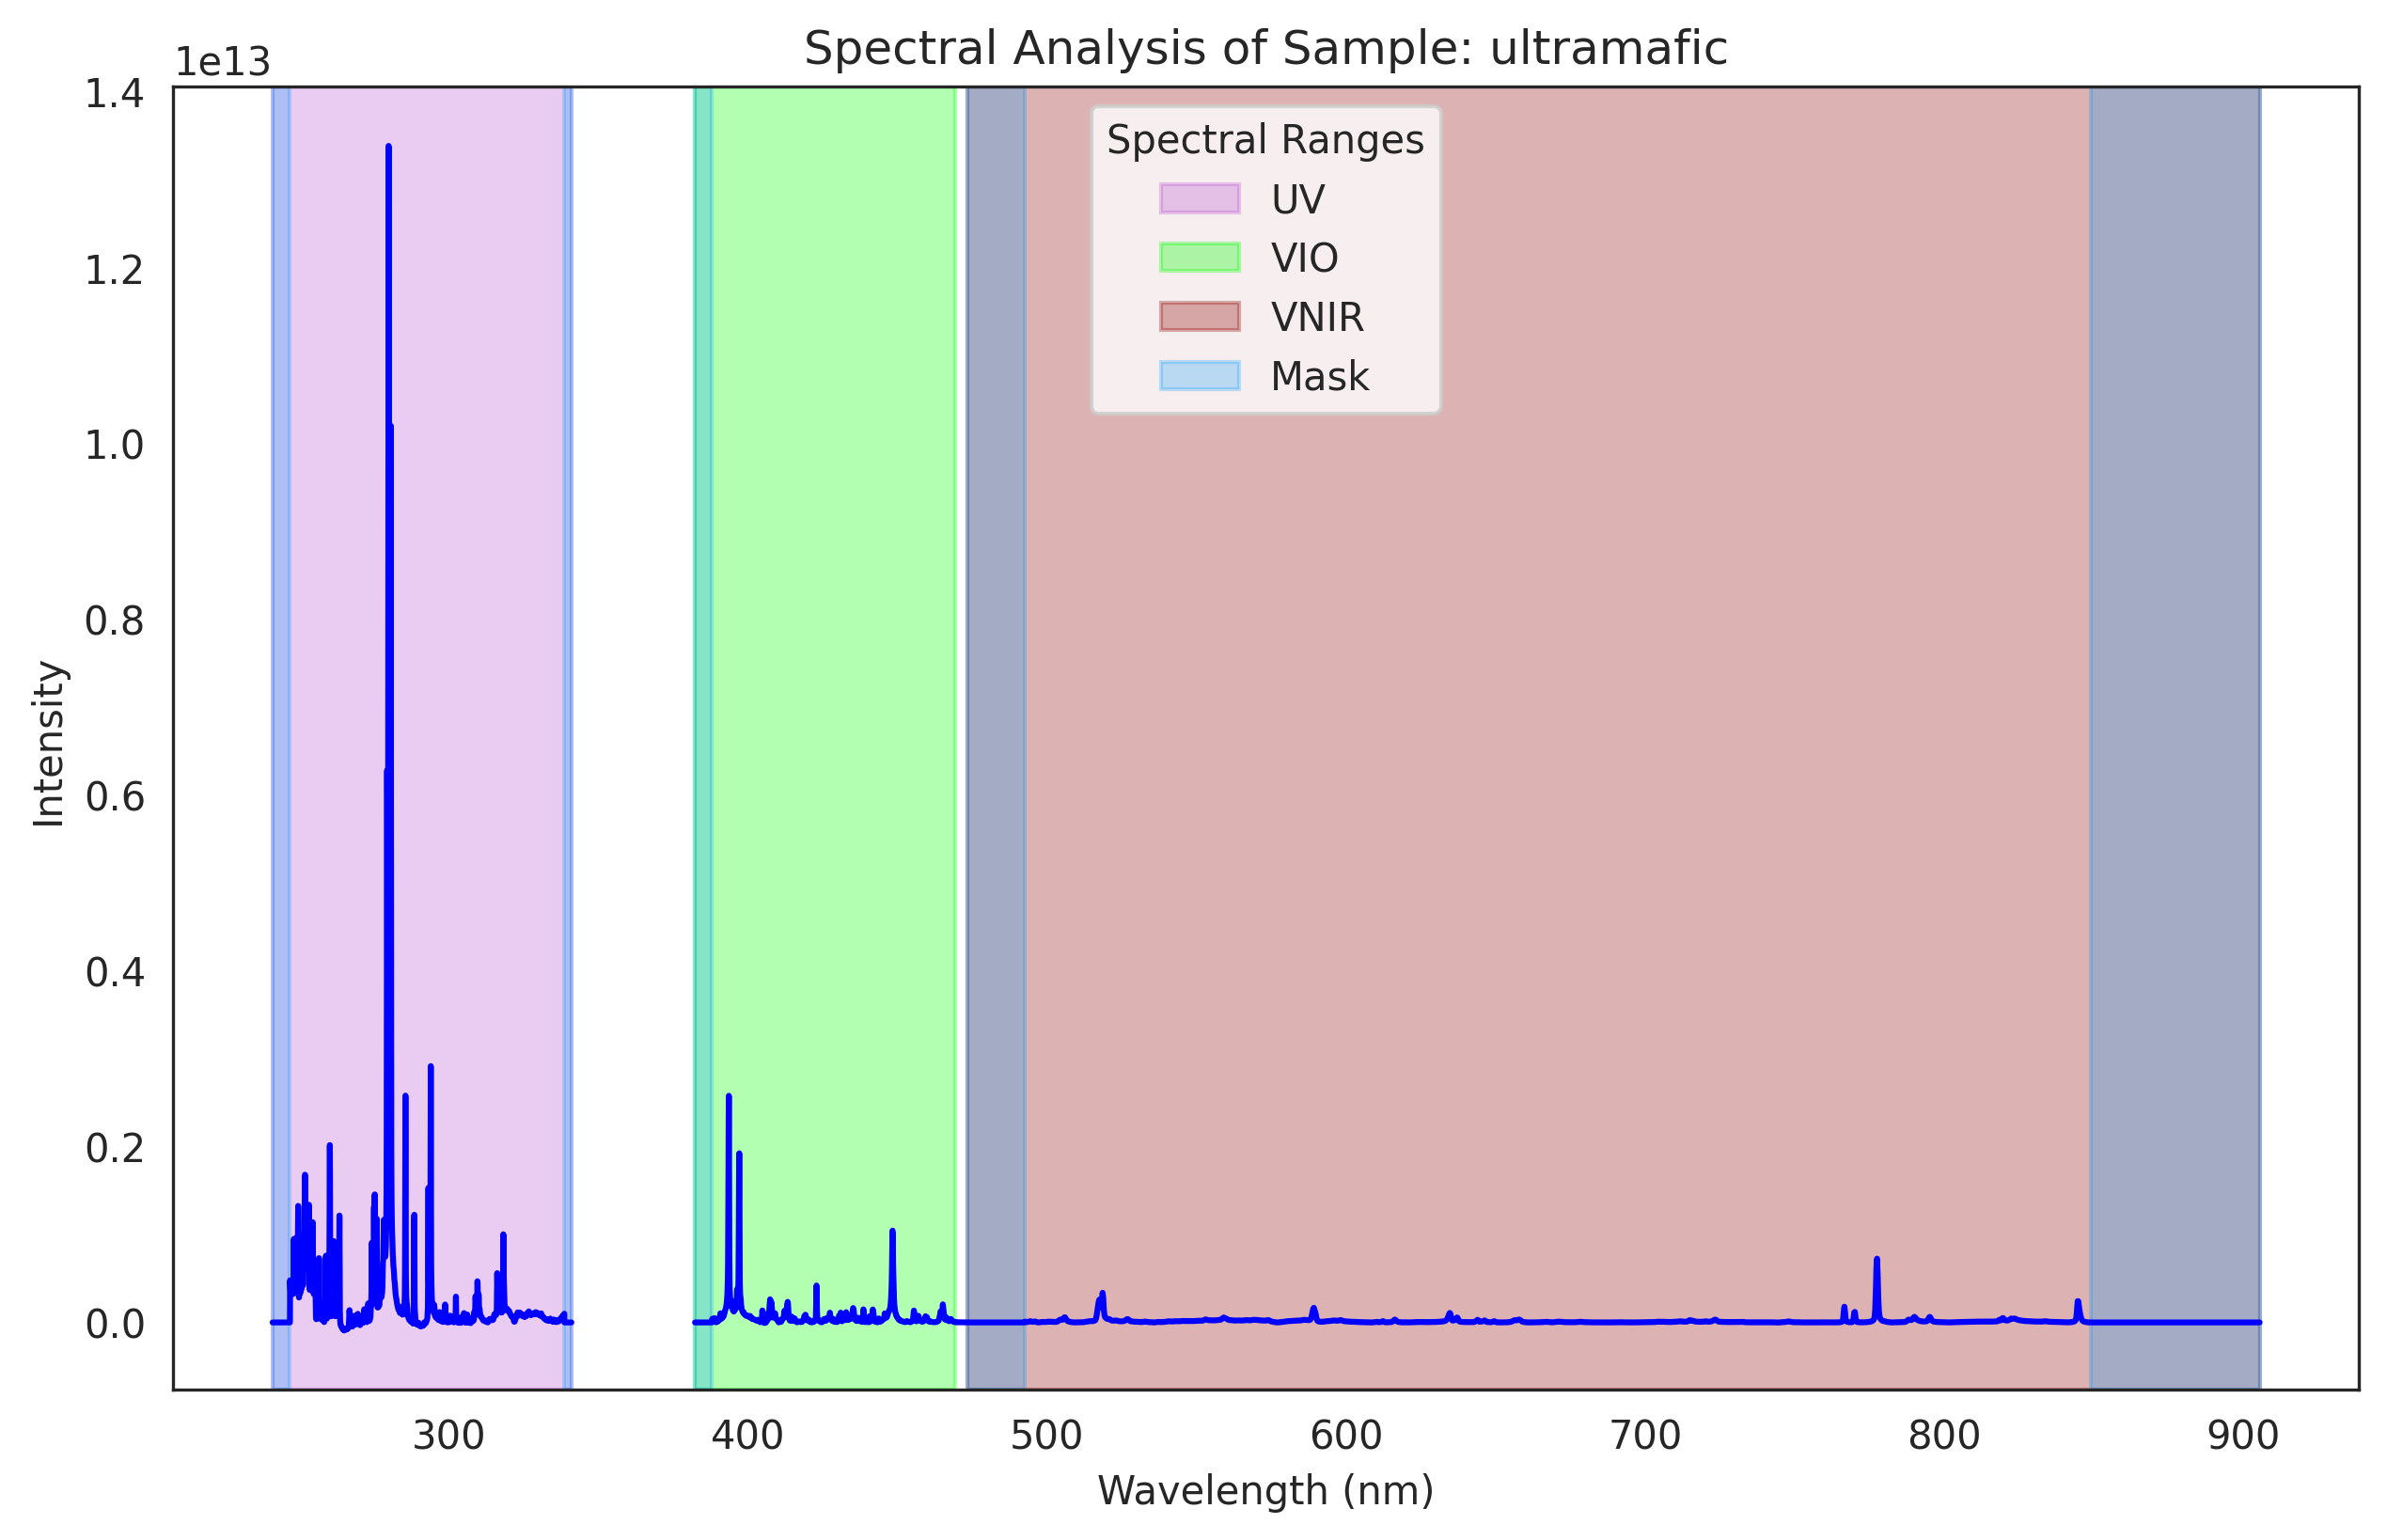
\includegraphics[width=0.5\textwidth]{images/spectral_plot.png}
	\caption{Spectral plot of the \gls{ccs} data for the \textit{ultramafic} sample. The wavelengths represent the spectral channels.}
	\label{fig:spectral_plot}
\end{figure}

Let $\gamma$ represent the spectrometer index, where $\gamma \in \{1, 2, 3\}$, corresponding to the \gls{uv}, \gls{vio}, and \gls{vnir} spectrometers, respectively.
Then, Norm 3 is formally defined as:

\begin{equation}
	\tilde{X}_{i,j}^{(\gamma)} = \frac{X_{i,j}^{(\gamma)}}{\sum_{j=1}^{N} X_{i,j}^{(\gamma)}},
\end{equation}

where

\begin{itemize}
	\item $\tilde{X}_{i,j}^{(\gamma)}$ is the normalized wavelength intensity for the $i$-th sample in the $j$-th channel on the $\gamma$-th spectrometer,
	\item $X_{i,j}^{(\gamma)}$ is the original wavelength intensity for the $i$-th sample in the $j$-th channel on the $\gamma$-th spectrometer, and
	\item $N = 2048$ is the number of channels in each spectrometer.
\end{itemize}

This normalization method results in a total of $3N = 6144$ normalized features for each sample, as each of the three spectrometers contributes 2048 channels.